\documentclass[11pt]{article}

\usepackage[margin=1in]{geometry}
\usepackage{amsmath,amssymb}
\usepackage{graphicx}
\usepackage{hyperref}
\usepackage{booktabs}
\usepackage{array}
\usepackage{enumitem}
\usepackage{times}

\title{Adaptive Stigmergic Oversight:\\
A Scalable Framework for Human Supervision of Large AI Agent Swarms}

\author{Carmelo Iaria\\
\textit{Synaptic AI Consulting}\\
\texttt{carmelo@synapticai.consulting}}

\date{March 2026}

\begin{document}

\maketitle

\begin{abstract}
The deployment of multi-agent AI systems faces a fundamental trilemma: achieving high throughput, maintaining meaningful human control, and leveraging full AI capability simultaneously. Existing paradigms---Human-in-the-Loop (HITL), Human-on-the-Loop (HOTL), and full autonomy---each sacrifice at least one of these dimensions. We present \emph{Adaptive Stigmergic Oversight} (ASO), a novel three-layer architecture that resolves this trilemma through the synthesis of intent-based delegation, stigmergic agent coordination, and exception-based review. Drawing on supervisory control theory, swarm intelligence principles, and recent empirical scaling research, ASO enables a single human operator to maintain strategic control over swarms of $N \gg 8$ agents while preserving $>89\%$ operational efficiency at $N=50$. We formalize the framework mathematically, derive performance bounds from cognitive load theory and fan-out models, specify eight evaluation metrics spanning human-centric, system-centric, and team-centric dimensions, and demonstrate applicability across software development, data science, financial analysis, and strategic intelligence domains. The framework includes a concrete proof-of-concept architecture for implementation in production coding environments.
\end{abstract}

\section{Introduction}

The rapid advancement of large language model (LLM) capabilities has enabled the emergence of \emph{agentic AI systems}---autonomous software agents that can decompose complex tasks, use tools, and coordinate with other agents to achieve goals. However, deploying such systems at scale introduces a critical coordination challenge: how can a human operator maintain meaningful oversight and strategic control over a large swarm of AI agents without becoming the system's throughput bottleneck?

\subsection{The Trilemma of Human--AI Collaboration}

Contemporary approaches to multi-agent AI supervision face an inescapable trilemma.

\paragraph{Human-in-the-Loop (HITL).} The human reviews every agent output before action. This maximizes control and accuracy but creates a severe throughput bottleneck. Empirical fan-out studies show effective human supervision typically caps at approximately $5$--$8$ agents~\cite{olsen2004fan,perkins2024fanout}.

\paragraph{Human-on-the-Loop (HOTL).} Agents act autonomously while the human monitors dashboards. This improves throughput but leads to the well-documented out-of-the-loop (OOTL) performance problem: situation awareness degrades, skill atrophy occurs, and humans become poor judges of when to intervene~\cite{endsley1995toward,bainbridge1983ironies}.

\paragraph{Full Autonomy.} Agents operate without human oversight. This maximizes throughput and AI capability utilization but can yield large error amplification factors in independent multi-agent systems and hallucination cascades in a significant fraction of enterprise deployments~\cite{kim2026scaling}.

Each paradigm sacrifices at least one critical dimension: HITL sacrifices throughput, HOTL sacrifices control, and full autonomy sacrifices reliability.

\subsection{Contributions}

We present \emph{Adaptive Stigmergic Oversight} (ASO), a principled framework that resolves the trilemma through three synergistic mechanisms:

\begin{enumerate}[label=(\roman*),leftmargin=*]
    \item \textbf{Intent-based delegation.} Humans specify high-level objectives with constraint envelopes rather than task sequences, operating at Parasuraman's decision-selection stage while agents handle information acquisition, analysis, and implementation~\cite{parasuraman2000model}.
    \item \textbf{Stigmergic coordination.} Agents coordinate through shared artifacts (code repositories, data pipelines, knowledge graphs) rather than direct message passing, reducing coordination complexity from $O(n^2)$ to $O(n)$~\cite{crowston2006stigmergy,heylighen2016stigmergy,li2025swarmsys}.
    \item \textbf{Exception-based review.} Validator agents assess outputs against constraint envelopes; only low-confidence cases escalate to human review, maintaining strategic engagement while avoiding the OOTL problem~\cite{parasuraman2000model,chen2025trust}.
\end{enumerate}

Our key contributions are:
\begin{itemize}[leftmargin=*]
    \item A formal mathematical model of ASO that derives effective fan-out from exception probability, cognitive budget allocation, and per-agent trust dynamics.
    \item A performance metrics taxonomy spanning eight dimensions, drawing on decades of human factors research.
    \item Cross-domain application designs for software development, data science, financial analysis, and strategic intelligence.
    \item A concrete proof-of-concept architecture for implementation in production AI coding environments.
\end{itemize}

\section{Related Work}

\subsection{Supervisory Control and Levels of Automation}

Sheridan and Verplank introduced a 10-level automation scale ranging from complete manual control to full computer authority. Parasuraman et al.\ extended this into a two-dimensional model decomposing automation into four information-processing stages---acquisition, analysis, decision, and action---each independently automatable~\cite{parasuraman2000model}. This supports stage-selective automation: high automation for information functions with moderate automation for decision functions.

Endsley developed a three-level model of situation awareness (SA)---perception, comprehension, and projection---and showed that intermediate levels of automation can preserve SA more effectively than either extreme~\cite{endsley1995toward}. Bainbridge's ``Ironies of Automation'' argued that capable automation paradoxically creates more operator challenges, particularly during rare interventions where mental models and skills have degraded~\cite{bainbridge1983ironies}.

\subsection{Scalability and Fan-Out Models}

Olsen and Goodrich formalized fan-out as
\begin{equation}
\mathrm{FO} = \frac{N_T}{N_T - I_T},
\end{equation}
where $N_T$ is neglect time (how long the system can run without human attention) and $I_T$ is interaction time per agent~\cite{olsen2004fan}. Perkins and Johnson revisited this model, explicitly incorporating human estimation error and showing that practical fan-out systematically underperforms theoretical predictions~\cite{perkins2024fanout}.

\subsection{Multi-Agent Systems and Coordination}

A recent empirical study from Google Research evaluated a large number of agent configurations across several architectures and tasks, finding that centralized coordination improves performance on parallelizable tasks but can degrade sequential reasoning and amplify error in certain regimes~\cite{kim2026scaling}. Error amplification was lowest under centralized orchestration and highest for independent agents.

Li et al.\ proposed SwarmSys, which applies stigmergy to LLM agents using Explorer, Worker, and Validator roles, outperforming baseline agent designs on symbolic reasoning and research synthesis tasks~\cite{li2025swarmsys}. Broader human--swarm interaction studies indicate that simple autonomous swarms excel in open environments while human guidance adds value in structured, safety-critical contexts.

\subsection{Adjustable Autonomy and Trust}

Scerri et al.\ developed mathematical foundations for adjustable autonomy in real-world multi-agent systems~\cite{scerri2002adjustable}. The KAoS policy framework operationalizes this via policy-bounded agent behavior and enforcement~\cite{bradshaw2004making}. Miller and Parasuraman introduced Playbook delegation concepts for supervisory control interfaces~\cite{miller2007flexible}.

Dynamic trust calibration approaches use learning-based methods to determine when to rely on automation and when to escalate to human review. Chen et al.\ model this as a contextual bandit problem, demonstrating higher rewards across experimental conditions~\cite{chen2025trust}.

\section{The ASO Framework}

\subsection{Architecture Overview}

ASO comprises three synergistic layers.

\paragraph{Layer 1: Intent-based delegation (Human $\rightarrow$ Swarm).} The human operator specifies \emph{intents}: high-level objectives with constraint envelopes defining acceptable boundaries for quality, risk, scope, and approach. An intent decomposer translates intents into policy-bounded work packages that define each agent's permissible action space.

\paragraph{Layer 2: Stigmergic swarm (Agent $\leftrightarrow$ Agent).} Agents coordinate through shared artifact spaces (e.g., code repositories, experiment tracking systems, knowledge graphs) rather than direct communication. Following stigmergic coordination patterns~\cite{crowston2006stigmergy,heylighen2016stigmergy}, this requires no explicit global plan or mutual awareness. Agents cycle through Explorer, Worker, and Validator roles with pheromone-like reinforcement signals embedded in the artifact space~\cite{li2025swarmsys}.

\paragraph{Layer 3: Exception-based review (Swarm $\rightarrow$ Human).} Validator agents assess every output against the constraint envelope. When confidence exceeds a threshold $\theta$, outputs are auto-approved and merged into the artifact space; those below $\theta$ escalate to human review with full context, confidence score, and validator reasoning.

\begin{figure}[t]
    \centering
    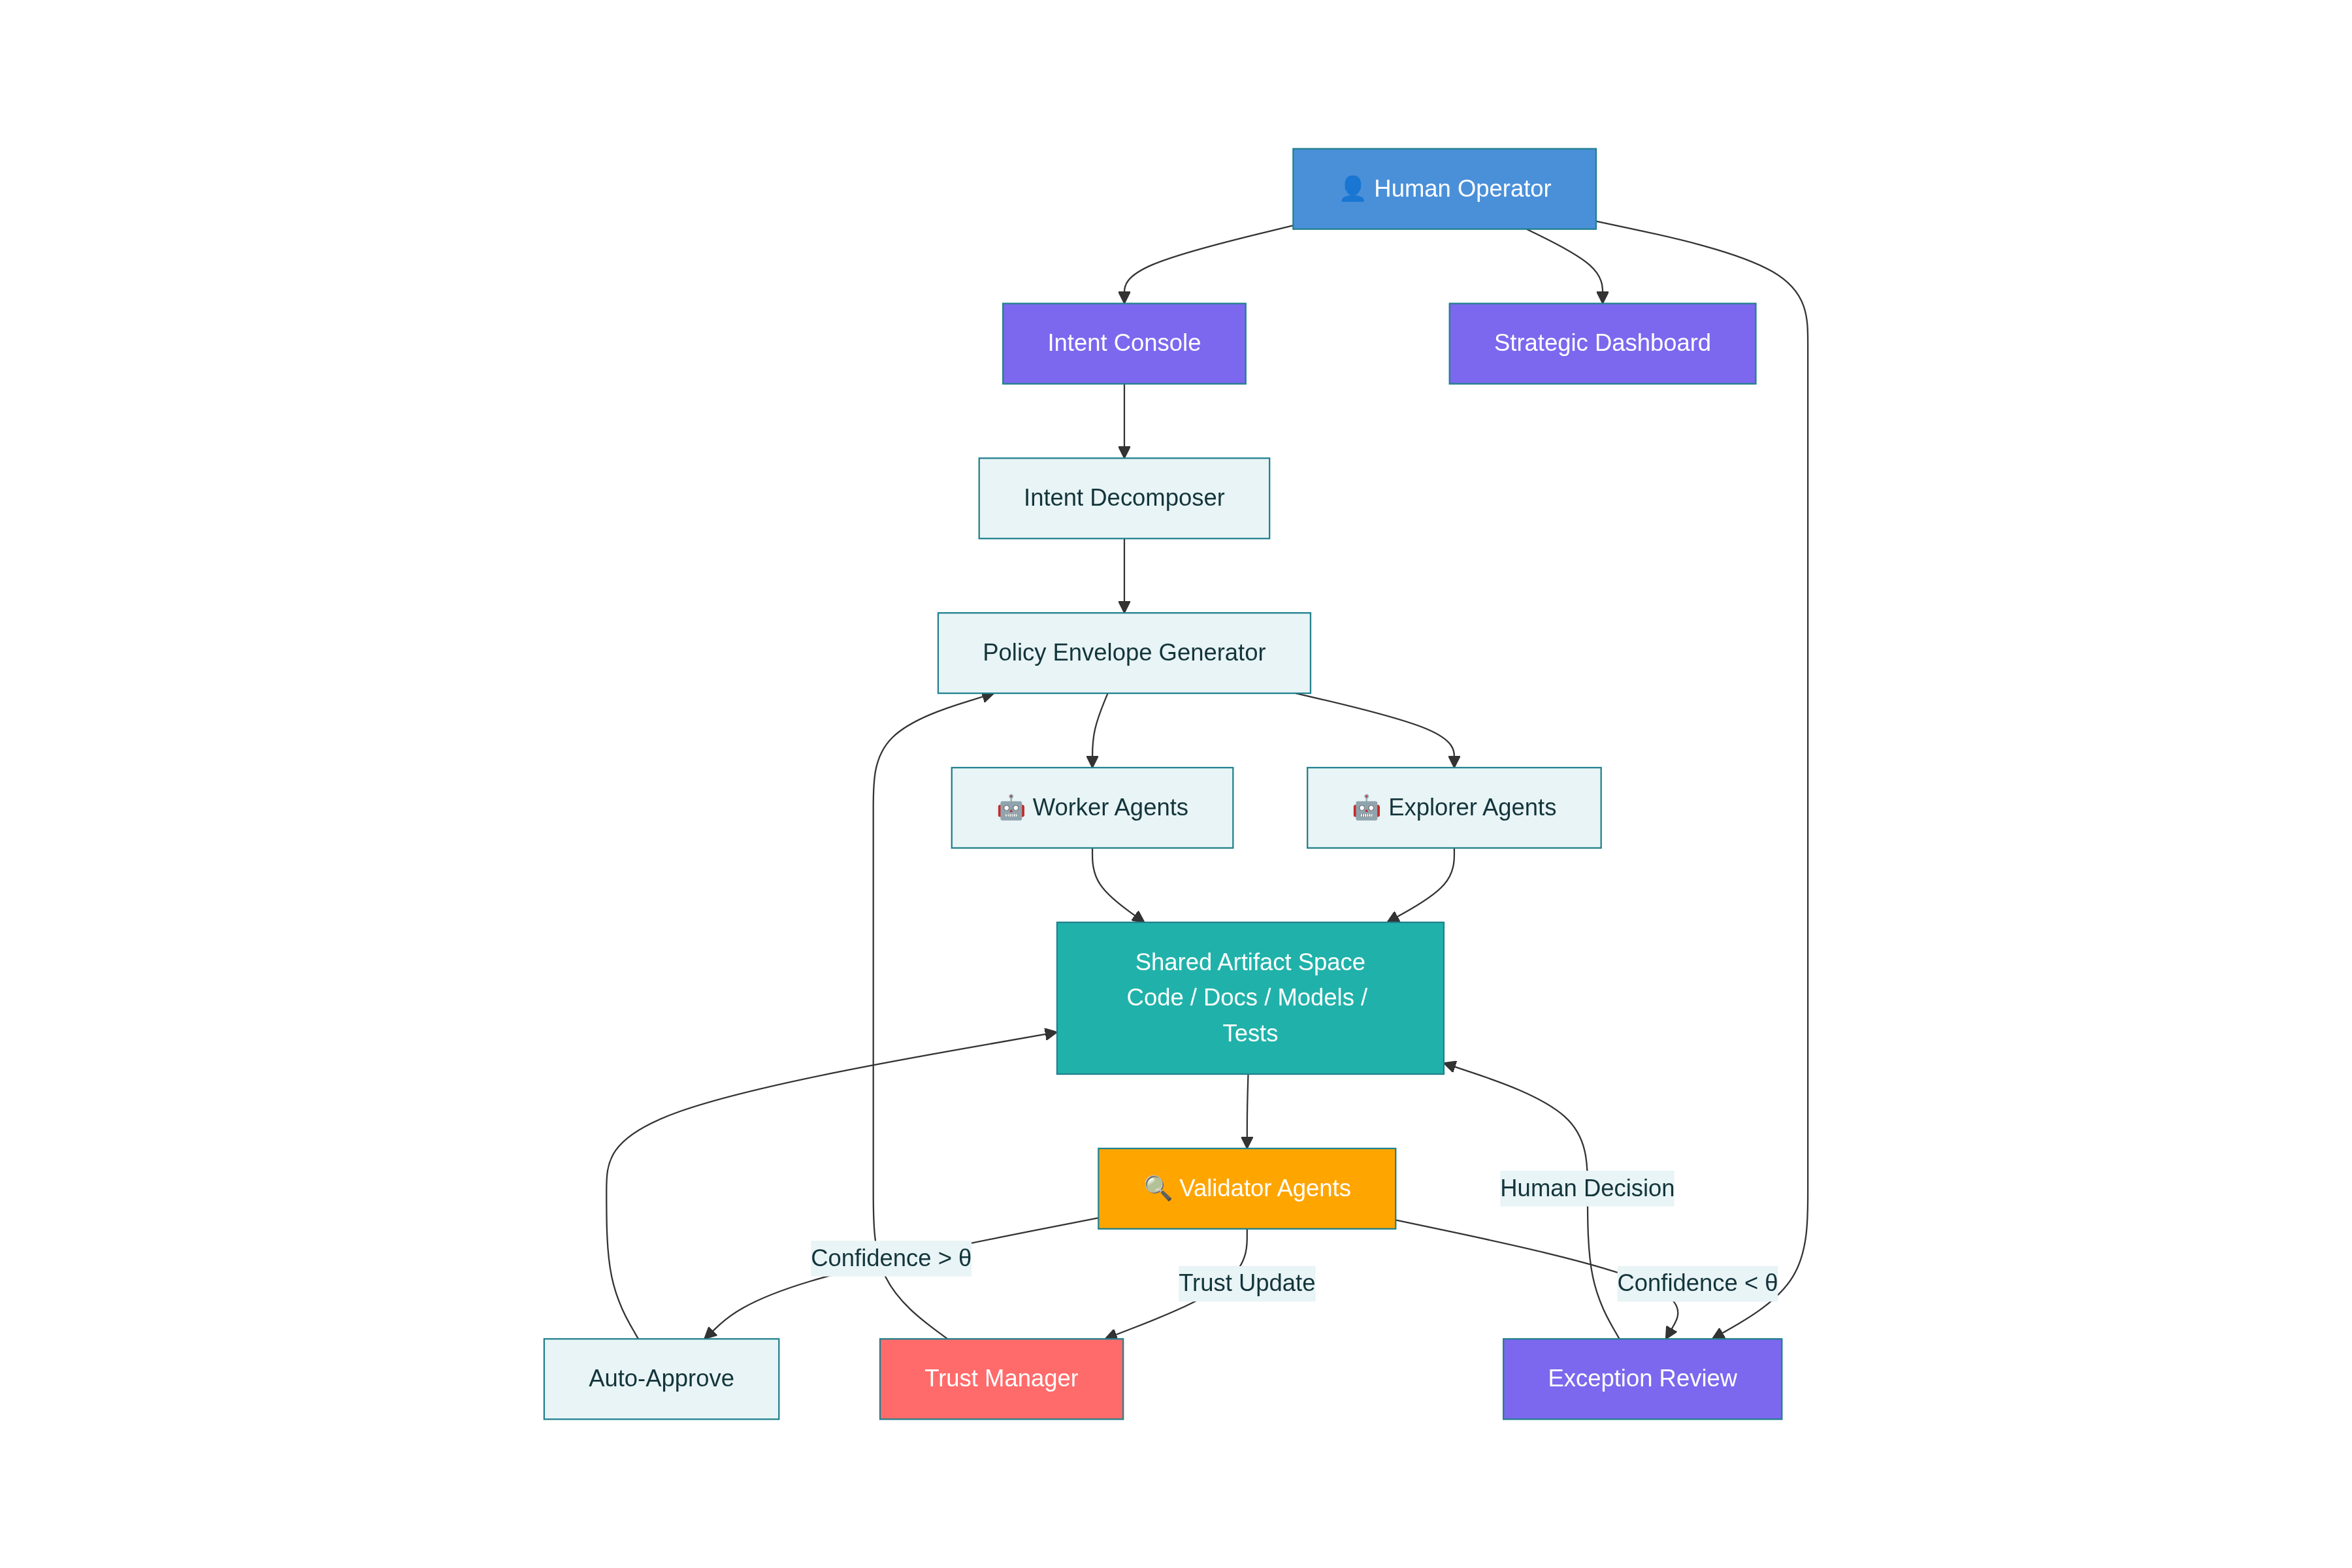
\includegraphics[width=0.9\textwidth]{figs/aso-architecture.png}
    \caption{High-level architecture of Adaptive Stigmergic Oversight (ASO), showing the flow from human intent through the stigmergic agent swarm to exception-based human review.}
    \label{fig:aso-architecture}
\end{figure}

\subsection{Mathematical Model}

\subsubsection{Effective Fan-Out}

We define effective fan-out under ASO as
\begin{equation}
\mathrm{FO}_{\text{ASO}} = N \left( 1 - P_e \frac{T_r}{T_c} \right),
\label{eq:foaso}
\end{equation}
where $N$ is total agent count, $P_e$ is the exception probability (fraction of outputs requiring human review), $T_r$ is time per exception review, and $T_c$ is the agent work cycle time. As $P_e \to 0$ through learning and trust calibration, $\mathrm{FO}_{\text{ASO}} \to N$.

\paragraph{Proposition 1.} For target exception rate $P_e = 0.08$, review time $T_r = 2$ minutes, and cycle time $T_c = 15$ minutes, ASO maintains approximately $89.3\%$ efficiency independent of $N$, assuming validator overhead remains negligible for $N < 100$.

\subsubsection{Cognitive Budget Allocation}

The human cognitive budget $C_{\text{total}}$ is allocated across:
\begin{equation}
C_{\text{intent}} + C_{\text{review}} + C_{\text{meta}} + C_{\text{redirect}} \leq C_{\text{total}},
\label{eq:cognitive}
\end{equation}
where $C_{\text{intent}}$ is effort devoted to formulating strategic intents, $C_{\text{review}} = P_e N c_{\text{per\_review}}$ is exception review load, $C_{\text{meta}}$ is monitoring swarm health, and $C_{\text{redirect}}$ is periodic strategic adjustment. The optimization goal is to maximize $C_{\text{intent}}$ subject to~\eqref{eq:cognitive}, primarily by reducing $C_{\text{review}}$ via lowering $P_e$.

\subsubsection{Dynamic Trust Calibration}

Each agent $i$ maintains a trust score $\tau_i(t)$ updated via exponential smoothing:
\begin{equation}
\tau_i(t+1) = \alpha \,\tau_i(t) + (1-\alpha)\, r_i(t),
\end{equation}
where $r_i(t) \in [0,1]$ is outcome quality and $\alpha \in (0,1)$ is a smoothing parameter. Constraint envelopes adapt based on trust tiers: high-trust agents (e.g., $\tau_i > \theta_{\text{high}}$) receive wider envelopes and less frequent review, while low-trust agents (e.g., $\tau_i < \theta_{\text{low}}$) operate under tighter envelopes with mandatory checkpoints.

\subsubsection{Coordination Complexity}

\paragraph{Theorem 1.} Stigmergic coordination via shared artifacts scales $O(n)$ in communication complexity, versus $O(n^2)$ for peer-to-peer message passing.

\paragraph{Sketch of proof.} In peer-to-peer coordination, each of $n$ agents may need to communicate with up to $n-1$ peers, yielding $O(n^2)$ message complexity. In stigmergic coordination, each agent reads from and writes to a shared artifact space in $O(1)$ per operation; for $n$ agents the total communication cost is $O(n)$~\cite{heylighen2016stigmergy}.

\section{Performance Metrics Framework}

We define eight evaluation metrics across human-centric, system-centric, and team-centric dimensions. Table~\ref{tab:metrics} summarizes targets and theoretical bases.

\begin{table}[t]
\centering
\begin{tabular}{p{3.0cm}p{2.0cm}p{2.5cm}p{5.0cm}}
\toprule
\textbf{Metric} & \textbf{Category} & \textbf{Target} & \textbf{Theoretical Basis} \\
\midrule
Swarm Throughput & System & Domain-specific & Multi-agent scaling results~\cite{kim2026scaling} \\
Exception Rate & System & $< 10\%$ & Trust calibration and validator design~\cite{chen2025trust} \\
Human Utilization & Human & $>70\%$ intent & Cognitive budget model, Eq.~\eqref{eq:cognitive} \\
Error Containment & Team & $<4.4 \times$ & Centralized orchestration baseline~\cite{kim2026scaling} \\
Intent Fidelity & Team & $>0.85$ cosine & Shared mental model theory and intent similarity \\
Coordination Cost & System & $<15\%$ overhead & $O(n)$ stigmergic bound, Theorem 1 \\
Adaptation Speed & Team & $T_{1/2} < 5$ cycles & Trust update dynamics \\
Time-to-Value & Team & Domain-specific & Fan-out model, Eq.~\eqref{eq:foaso} \\
\bottomrule
\end{tabular}
\caption{Performance metrics for evaluating Adaptive Stigmergic Oversight.}
\label{tab:metrics}
\end{table}

\begin{figure}[t]
    \centering
    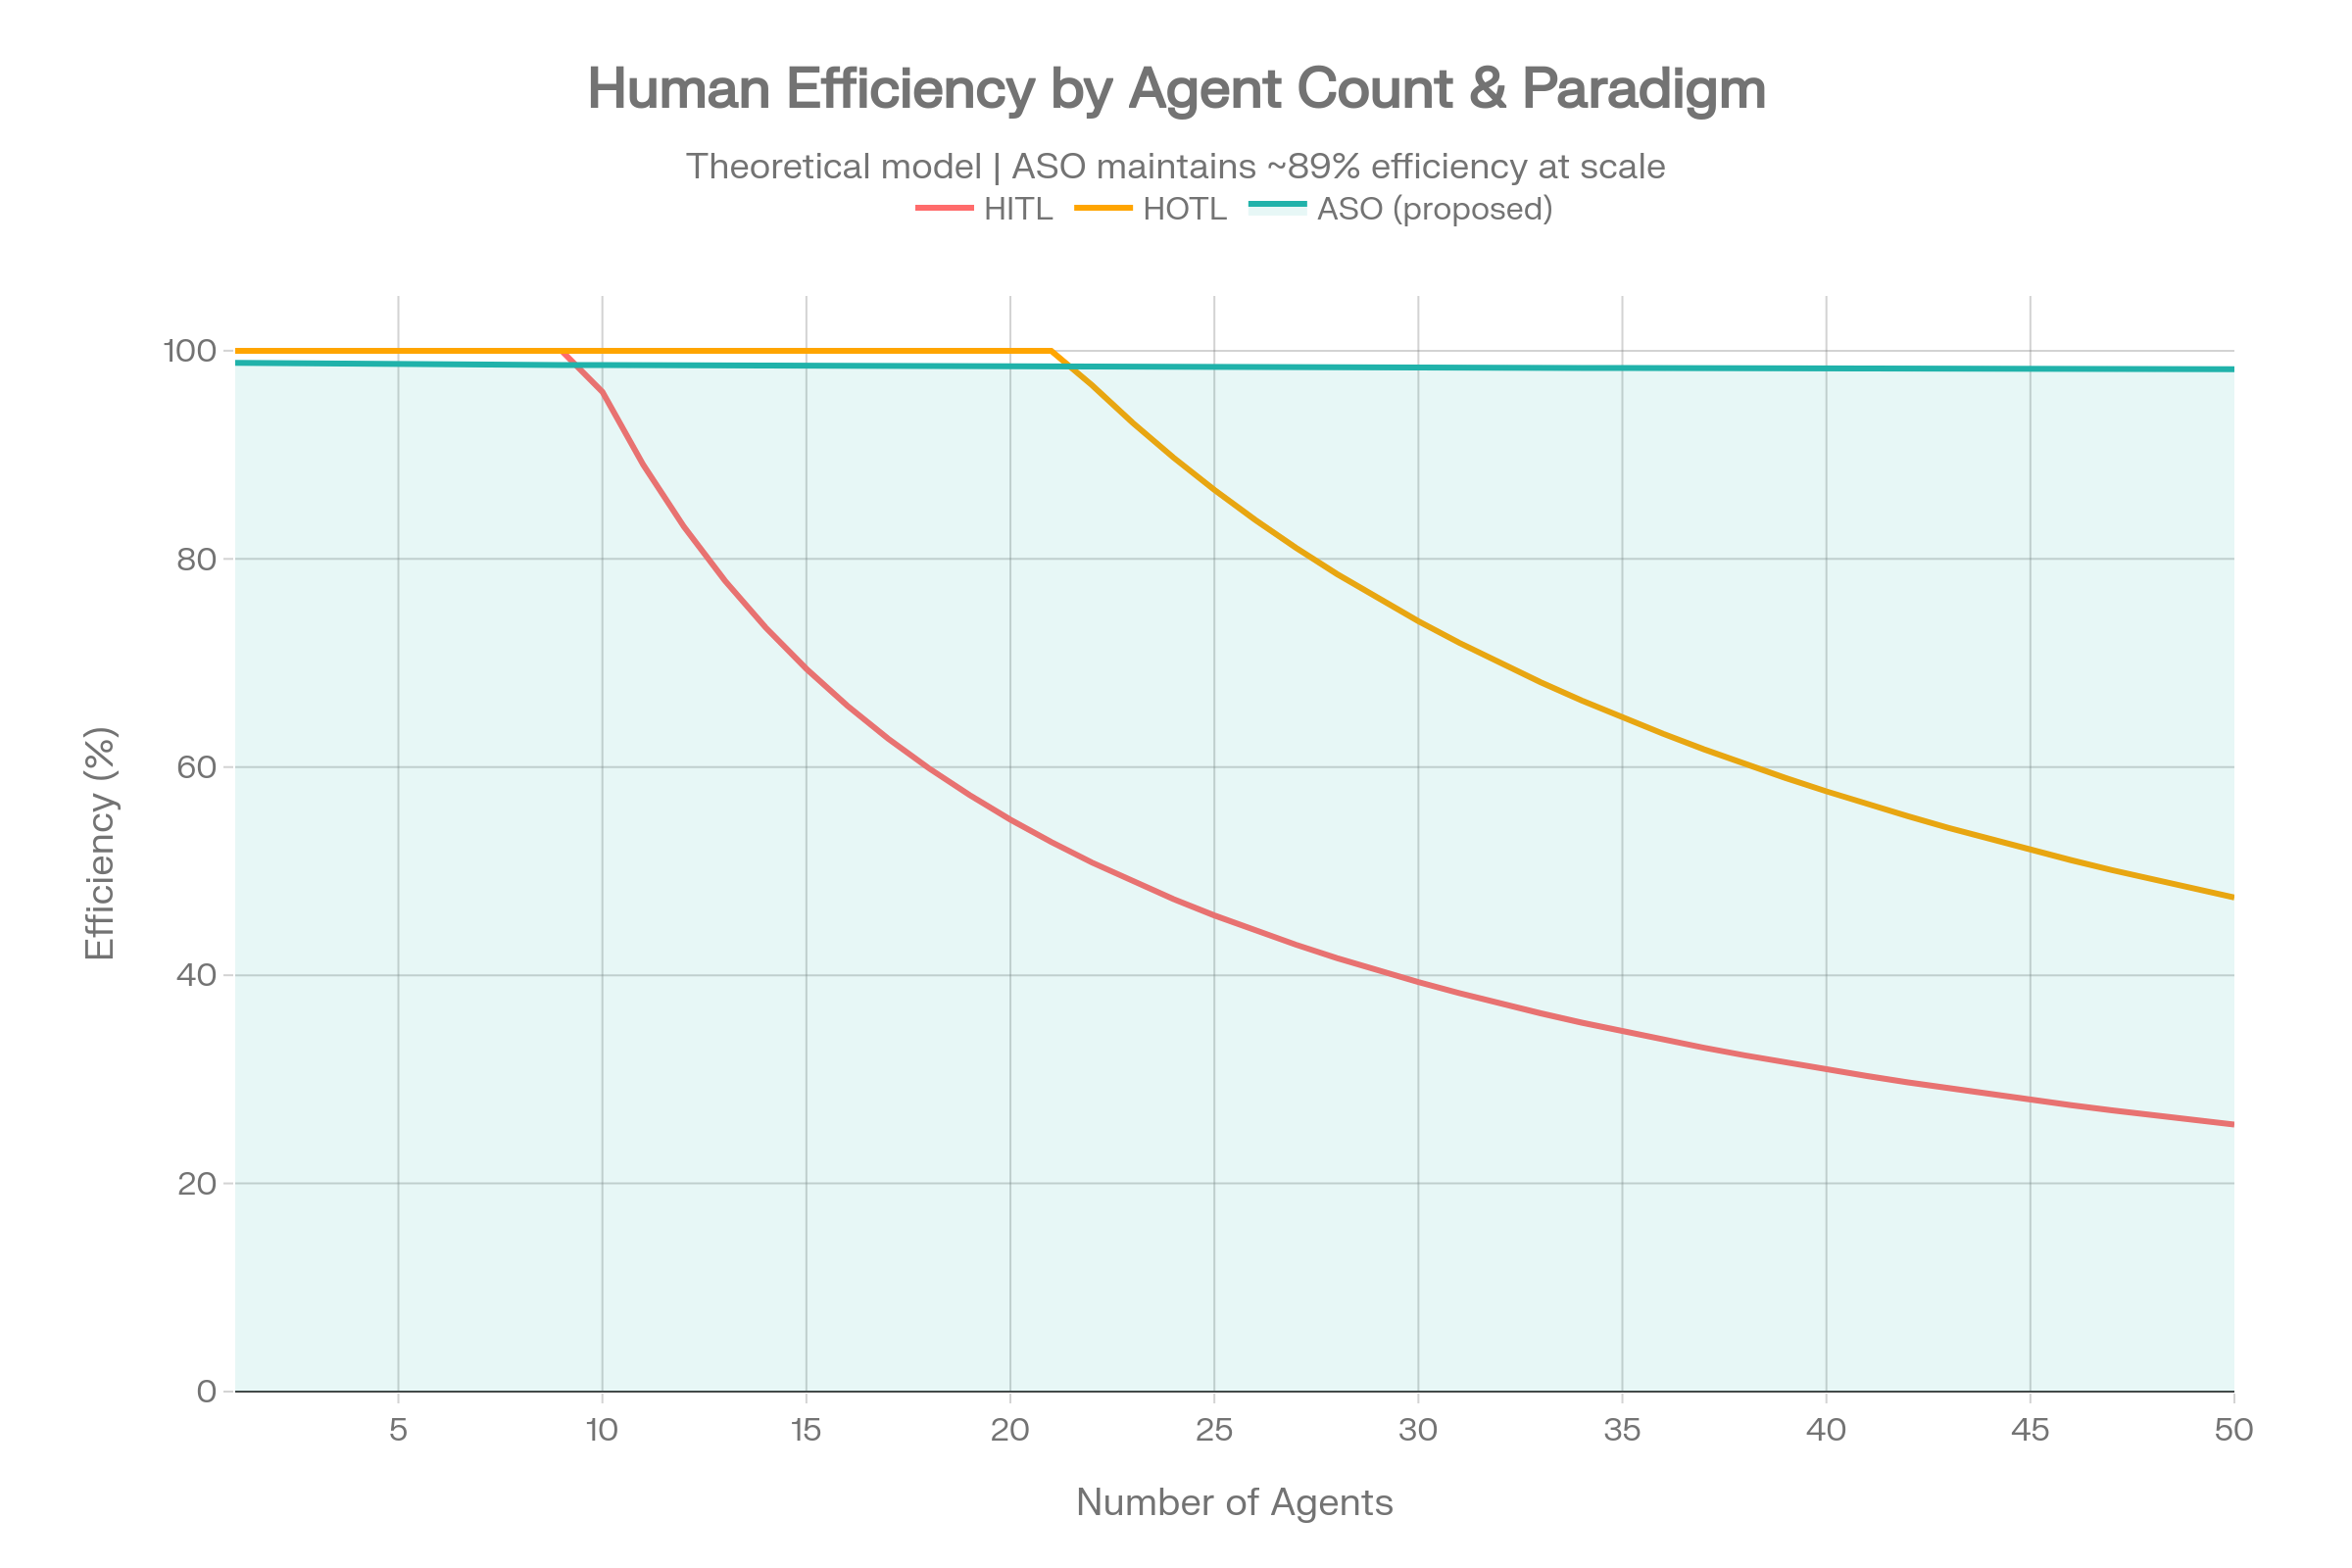
\includegraphics[width=0.7\textwidth]{figs/aso-fanout.png}
    \caption{Illustrative comparison of human efficiency across paradigms as the number of agents increases: HITL degrades quickly, HOTL degrades more slowly, while ASO maintains high efficiency at scale.}
    \label{fig:aso-fanout}
\end{figure}

\section{Cross-Domain Applications}

\subsection{Software Development}

\textbf{Intent example.} Implement OAuth2 authentication supporting Google and GitHub providers, with $90\%+$ test coverage and OpenAPI documentation.

\textbf{Constraint envelope.} Use the existing authentication library; follow project coding standards; do not modify database schema; all continuous integration (CI) checks must pass.

\textbf{Stigmergic medium.} Git repository, CI/CD pipeline, test results, and linter output.

\textbf{Agent roles.} Feature implementers, test writers, documentation generators, security scanners, and integration validators. Exception triggers include failing CI, security vulnerabilities, architectural deviations, or coverage below threshold.

\subsection{Data Science}

\textbf{Intent example.} Build a churn prediction model for the Q1 cohort, comparing ensemble and deep learning approaches, with SHAP explanations and area under the ROC curve (AUC) greater than $0.82$.

\textbf{Constraint envelope.} Only approved data sources; inference latency below $100$ ms; no personally identifiable information in features.

\textbf{Stigmergic medium.} Experiment tracking (e.g., MLflow), feature store, and model registry. Exception triggers include data drift, performance anomalies, or inconsistent feature importance patterns.

\subsection{Financial Analysis}

\textbf{Intent example.} Perform discounted cash flow (DCF) valuation of acquisition target $X$ with comparable company analysis and bear/base/bull scenarios.

\textbf{Constraint envelope.} Use only official filings; cite all assumptions; flag cases where valuation is more than $20\%$ sensitive to any single key variable.

\textbf{Stigmergic medium.} Shared financial models, assumption registry, and citation graph. Exceptions arise from contradictory data, high sensitivity, or missing disclosures.

\subsection{Strategic Intelligence}

\textbf{Intent example.} Map the competitive landscape for enterprise AI orchestration, identifying the top ten players, differentiation, and market gaps.

\textbf{Constraint envelope.} Use sources from 2025 onward; include both public and analyst perspectives; explicitly distinguish speculation from verified facts.

\textbf{Stigmergic medium.} Knowledge graph, competitive matrix, and evidence repository. Exceptions are triggered by conflicting data, novel competitor signals, or material information gaps.

\section{Proof of Concept: Cursor Implementation}

Cursor supports parallel AI agents operating over software repositories with features such as git worktree isolation and integrated testing pipelines. Recent work reports that a substantial fraction of Cursor's own merged pull requests originate from autonomous agents, with plan--build--review cycles scaling to thousands of commits and over a million lines of code~\cite{cursor2026scaling}.

\subsection{Implementation Architecture}

\textbf{Intent console.} A custom command or configuration file (e.g., YAML) defines intents, constraint envelopes, and trust thresholds. For example:
\begin{quote}
\texttt{intent: ``Implement notification system''}\\
\texttt{constraints: event-driven, existing bus; unit and integration tests with $>85\%$ coverage; latency $<200$ ms; no auth/billing changes}\\
\texttt{trust\_thresholds: auto\_approve 0.85; escalate 0.60; block 0.40}
\end{quote}

\textbf{Agent swarm.} Git worktrees provide isolated workspaces. Each agent reads from and writes to the shared repository (the stigmergic medium), following role-specific policies.

\textbf{Validator agents.} Dedicated validator agents execute test suites, linters, and security scans, compute confidence scores, and either auto-merge changes or create flagged pull requests for human review.

\textbf{Trust manager.} A persistent store tracks per-agent trust scores, updated after each cycle. Constraint envelopes are widened or narrowed based on trust tiers, implementing dynamic adjustable autonomy~\cite{scerri2002adjustable,chen2025trust}.

\section{Discussion}

\subsection{Comparison to Existing Paradigms}

Table~\ref{tab:comparison} contrasts ASO with HITL, HOTL, and full autonomy along several dimensions.

\begin{table}[t]
\centering
\begin{tabular}{p{3.0cm}p{2.0cm}p{2.0cm}p{2.5cm}p{2.0cm}}
\toprule
\textbf{Dimension} & \textbf{HITL} & \textbf{HOTL} & \textbf{Full Autonomy} & \textbf{ASO} \\
\midrule
Throughput & Low & High & High & High \\
Human Control & High & Low & None & High \\
Error Containment & High & Medium & Low & High \\
Cognitive Load & High & Low & Low & Medium \\
Situation Awareness & High & Low & N/A & High \\
Scalability ($N$) & $5$--$8$ & $20$--$30$ & Unlimited & $50+$ \\
\bottomrule
\end{tabular}
\caption{Qualitative comparison of oversight paradigms.}
\label{tab:comparison}
\end{table}

\begin{figure}[t]
    \centering
    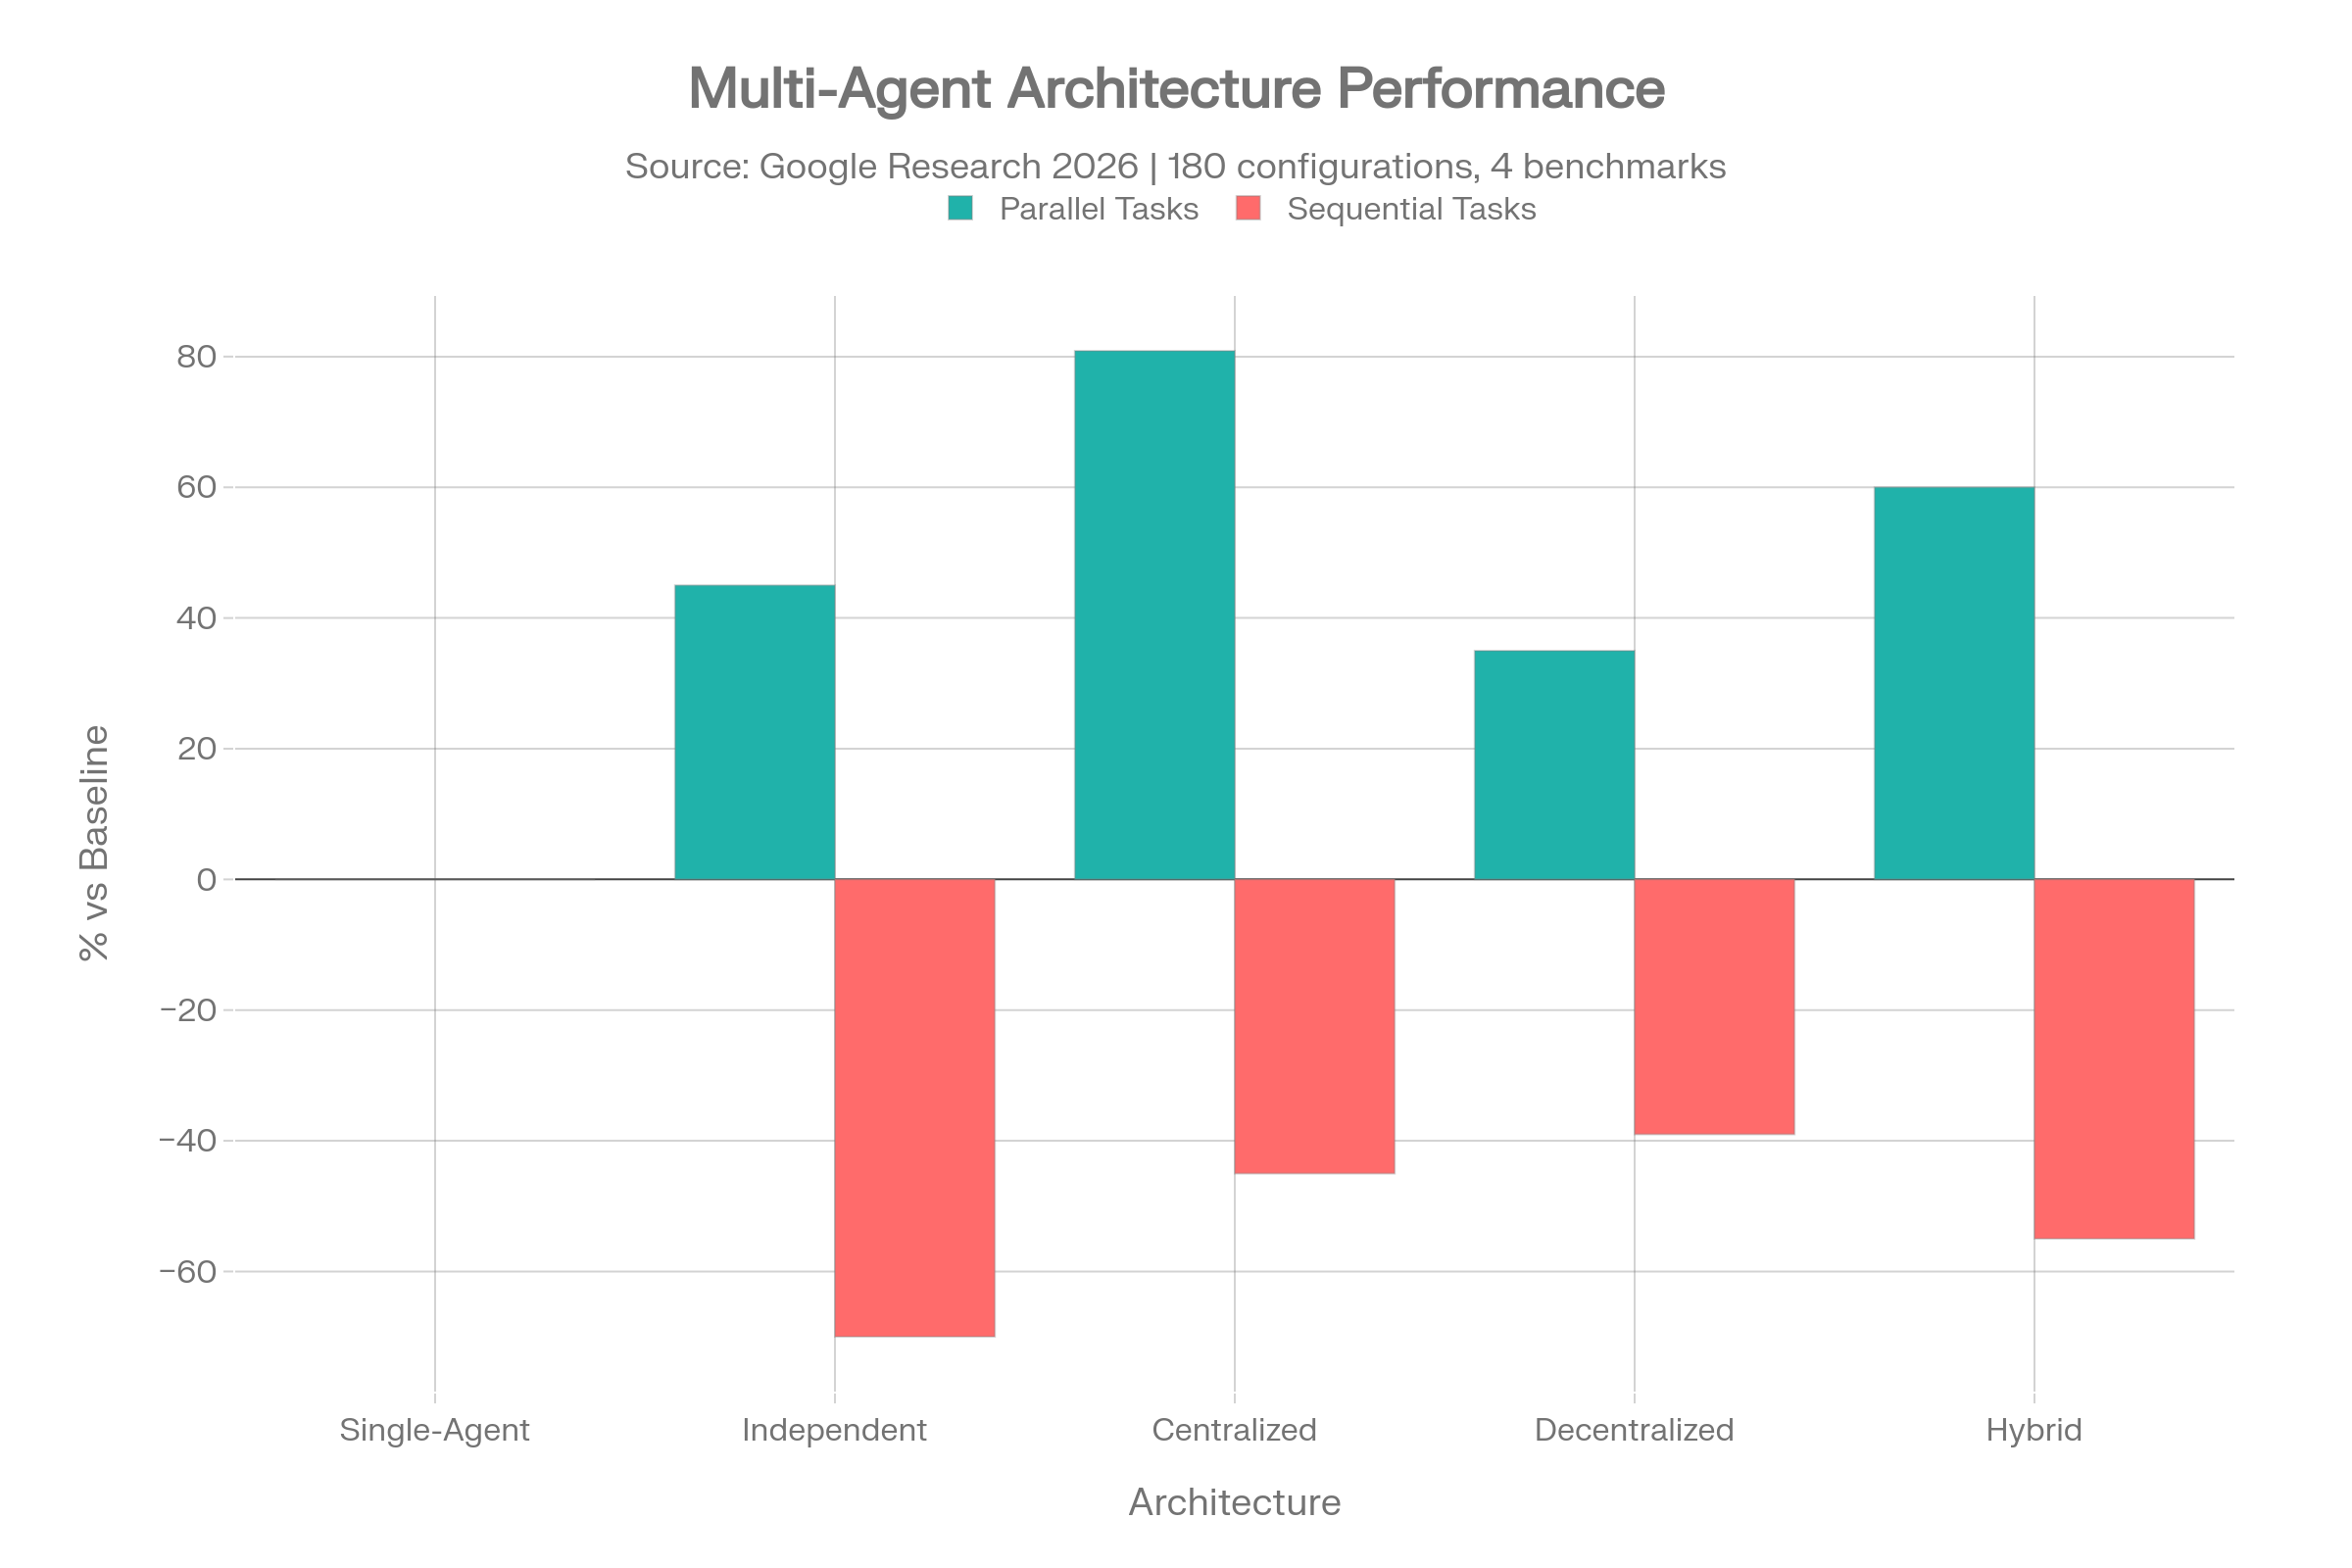
\includegraphics[width=0.9\textwidth]{figs/arch-performance.png}
    \caption{Performance of different multi-agent architectures on parallel and sequential tasks, illustrating trade-offs between independent, centralized, and hybrid coordination strategies.}
    \label{fig:arch-performance}
\end{figure}

ASO combines high throughput with high control and strong error containment by situating the human at the strategic layer (intent and exceptions) while agents execute within policy bounds. HITL systems lack stigmergic scaling; fully autonomous swarms lack principled oversight; centralized orchestrators risk bottlenecks and context loss.

\subsection{Theoretical Novelty}

ASO synthesizes three independently validated mechanisms:
\begin{enumerate}[label=(\alph*),leftmargin=*]
    \item Stage-selective automation from supervisory control~\cite{parasuraman2000model}.
    \item Stigmergic $O(n)$ coordination from swarm intelligence~\cite{heylighen2016stigmergy,li2025swarmsys}.
    \item Dynamic per-agent trust with policy-bounded envelopes from adjustable autonomy~\cite{scerri2002adjustable,chen2025trust}.
\end{enumerate}
To our knowledge, no prior framework combines all three in a unified model for supervising large LLM-based agent swarms.

\subsection{Limitations and Future Work}

ASO assumes that validator agents can accurately assess output quality and estimate confidence; if validators are unreliable, exception rates may be miscalibrated. Future work includes meta-validation and ensemble validator designs.

Translating human intent into formal constraint envelopes requires domain expertise and may introduce specification errors. Research on intent-to-policy compilers and interactive refinement interfaces is needed.

While we sketch applications across four domains, empirical validation is required to confirm that metric targets hold universally versus requiring domain-specific tuning. Finally, the framework does not directly address adversarial agents or Byzantine failures; integrating cryptographic verification and anomaly detection remains an important direction for production deployments.

\section{Conclusion}

Adaptive Stigmergic Oversight addresses the trilemma of human--AI collaboration at scale by enabling a single operator to maintain strategic control over swarms of $50+$ agents while preserving high operational efficiency. Through intent-based delegation, stigmergic coordination, and exception-based review, ASO positions the human in roles that exploit cognitive strengths while allowing agents to operate autonomously within adaptive policy bounds. The framework is grounded in human factors research and recent multi-agent scaling results and includes a proof-of-concept architecture suitable for real-world coding environments. Future work will focus on empirical evaluation across multiple domains and on extending ASO to address validator reliability, intent specification tooling, and adversarial robustness.

\begin{thebibliography}{99}

\bibitem{kim2026scaling}
J.~Kim et~al.
\newblock Towards a science of scaling agent systems: When and why agent systems work.
\newblock Google Research, 2026.

\bibitem{cursor2026scaling}
Cursor Team.
\newblock Scaling long-running autonomous coding.
\newblock Cursor Blog, 2026.

\bibitem{olsen2004fan}
D.~R. Olsen and M.~A. Goodrich.
\newblock Fan-out: Measuring human control of multiple robots.
\newblock In \emph{Proceedings of CHI}, 2004.

\bibitem{perkins2024fanout}
S.~Perkins and A.~Johnson.
\newblock Fan-out revisited: The impact of the human element on scalability of human multi-robot teams.
\newblock In \emph{Proceedings of ICRA}, 2024.

\bibitem{endsley1995toward}
M.~R. Endsley.
\newblock Toward a theory of situation awareness in dynamic systems.
\newblock \emph{Human Factors}, 37(1):32--64, 1995.

\bibitem{bainbridge1983ironies}
L.~Bainbridge.
\newblock Ironies of automation.
\newblock \emph{Automatica}, 19(6):775--779, 1983.

\bibitem{parasuraman2000model}
R.~Parasuraman, T.~B. Sheridan, and C.~D. Wickens.
\newblock A model for types and levels of human interaction with automation.
\newblock \emph{IEEE Transactions on Systems, Man, and Cybernetics--A}, 30(3):286--297, 2000.

\bibitem{crowston2006stigmergy}
K.~Crowston et~al.
\newblock The under-appreciated role of stigmergic coordination in open source software development.
\newblock In \emph{Proceedings of GROUP}, 2006.

\bibitem{heylighen2016stigmergy}
F.~Heylighen.
\newblock Stigmergy as a universal coordination mechanism.
\newblock \emph{Cognitive Systems Research}, 38:4--13, 2016.

\bibitem{li2025swarmsys}
X.~Li et~al.
\newblock SwarmSys: Decentralized swarm-inspired agents for scalable and adaptive reasoning.
\newblock arXiv:2510.10047, 2025.

\bibitem{scerri2002adjustable}
P.~Scerri et~al.
\newblock Towards adjustable autonomy for the real world.
\newblock \emph{Journal of Artificial Intelligence Research}, 17:171--228, 2002.

\bibitem{bradshaw2004making}
J.~M. Bradshaw et~al.
\newblock Making agents acceptable to people.
\newblock \emph{AI Magazine}, 25(3):29--47, 2004.

\bibitem{miller2007flexible}
C.~A. Miller and R.~Parasuraman.
\newblock Designing for flexible interaction between humans and automation: Delegation interfaces for supervisory control.
\newblock \emph{Human Factors}, 49(1):57--75, 2007.

\bibitem{chen2025trust}
J.~Chen et~al.
\newblock Trust calibration as contextual bandits for human--AI teams.
\newblock In \emph{Proceedings of CHI}, 2025.

\end{thebibliography}
\end{document}
